% ====================================================================
%  SECCIONES 8–13
% ====================================================================

\section{Modelo de Datos}

\subsection{Resumen del modelo}
\begin{center}
\begin{tabular}{|L{3.4cm}|L{11.6cm}|}
\hline
\thd{Propiedad} & \thd{Valor} \\
\hline
Motor & PostgreSQL 16 + extensión pgvector (base de datos vectorizada que sustenta el RAG) \\
\hline
Driver / acceso & AsyncPG (motor async de SQLAlchemy hacia PostgreSQL) \\
\hline
Arquitectura & Monolito modular \\
\hline
Total de tablas & 13 \\
\hline
Origen del diseño & ERD «Diagrama Entidad--Relación · IGUALAB --- Modelo de Datos Depurado» entregado por el equipo, con las correcciones aplicadas tras su revisión (puntos anotados en cada ficha) \\
\hline
Alcance retirado & Se retiraron 5 tablas del diseño v2 (configuración, catálogo de roles, medidor LLM separado) y se añadieron 4 nuevas \\
\hline
\end{tabular}
\end{center}

\subsection{El modelo por dominios (6 dominios --- refleja el ERD vigente)}
\begin{center}
\begin{tabular}{|L{3.2cm}|L{4.6cm}|L{6.7cm}|}
\hline
\thd{Dominio} & \thd{Tablas} & \thd{Propósito} \\
\hline
IDENTIDAD Y ACCESO & usuarios · sesiones · tokens\_recuperacion & Accounts of access, sesiones explícitas (JWT/sid) y recuperación de contraseña single-use. \\
\hline
EMPRESAS E INGESTA & empresas · documentos · fragmentos\_documento & Cadena de contenido fuente: catálogo de empresas, pipeline de ingesta .md y fragmentos vectorizados. \\
\hline
ANÁLISIS GRI & catalogo\_gri · gri\_analisis · sanciones & El estándar GRI (referencia) y la tabla única de resultados del análisis (códigos, citas, sanciones). \\
\hline
ASISTENTE RAG & consultas\_asistente · consulta\_citas & Persistencia de cada consulta al RAG con sus citas · fuentes (post-verificación de IDs). \\
\hline
REPORTES & reportes\_prospeccion & Entregable PDF inmutable + snapshot JSONB congelado a la fecha de emisión. \\
\hline
AUDITORÍA & auditoria & Bitácora append-only de eventos sensibles (solo INSERT; UTC). \\
\hline
\end{tabular}
\end{center}

\subsection{Entidades y relaciones (modelo conceptual)}
Cadena principal del negocio:

\noindent empresa $\rightarrow$ documento (.md) $\rightarrow$ fragmentos (vectorizados) $\rightarrow$ gri\_analisis $\rightarrow$ reportes\_prospeccion,\\
con: usuarios (quién hace qué) · auditoria (eventos sensibles) · catalogo\_gri (El estándar), consultas\_asistente + consulta\_citas (Asistente RAG).

Relaciones (todas 1:N salvo indicación):

\begin{enumerate}[leftmargin=1.6em,itemsep=2pt,topsep=2pt]
  \item Un usuario abre muchas sesiones y crea muchos tokens\_recuperacion.
  \item Una empresa tiene muchos documentos; un usuario crea los documentos (creado\_por).
  \item Un documento se vectoriza en muchos fragmentos\_documento; un documento produce muchas filas de gri\_analisis y cita muchas sanciones.
  \item Cada fila de gri\_analisis referencia un código del catalogo\_gri y proviene de un fragmento (fragmento\_id --- cita verificable).
  \item Una consulta\_asistente registra sus citas (consulta\_citas) enlazadas a fragmentos.
  \item Un reporte de prospección pertenece a una empresa (UNIQUE empresa+anio --- RN-041) y congela su snapshot a la fecha de emisión.
  \item Todo evento sensible registra auditoria (append-only; FK usuario/empresa NULL cuando aplica).
\end{enumerate}

\subsection{Diagrama Entidad--Relación (ERD vigente)}
ERD «Modelo de Datos Depurado» (13 tablas). El diagrama anterior Diagrama\_bd.png queda como archivo histórico.

\begin{center}
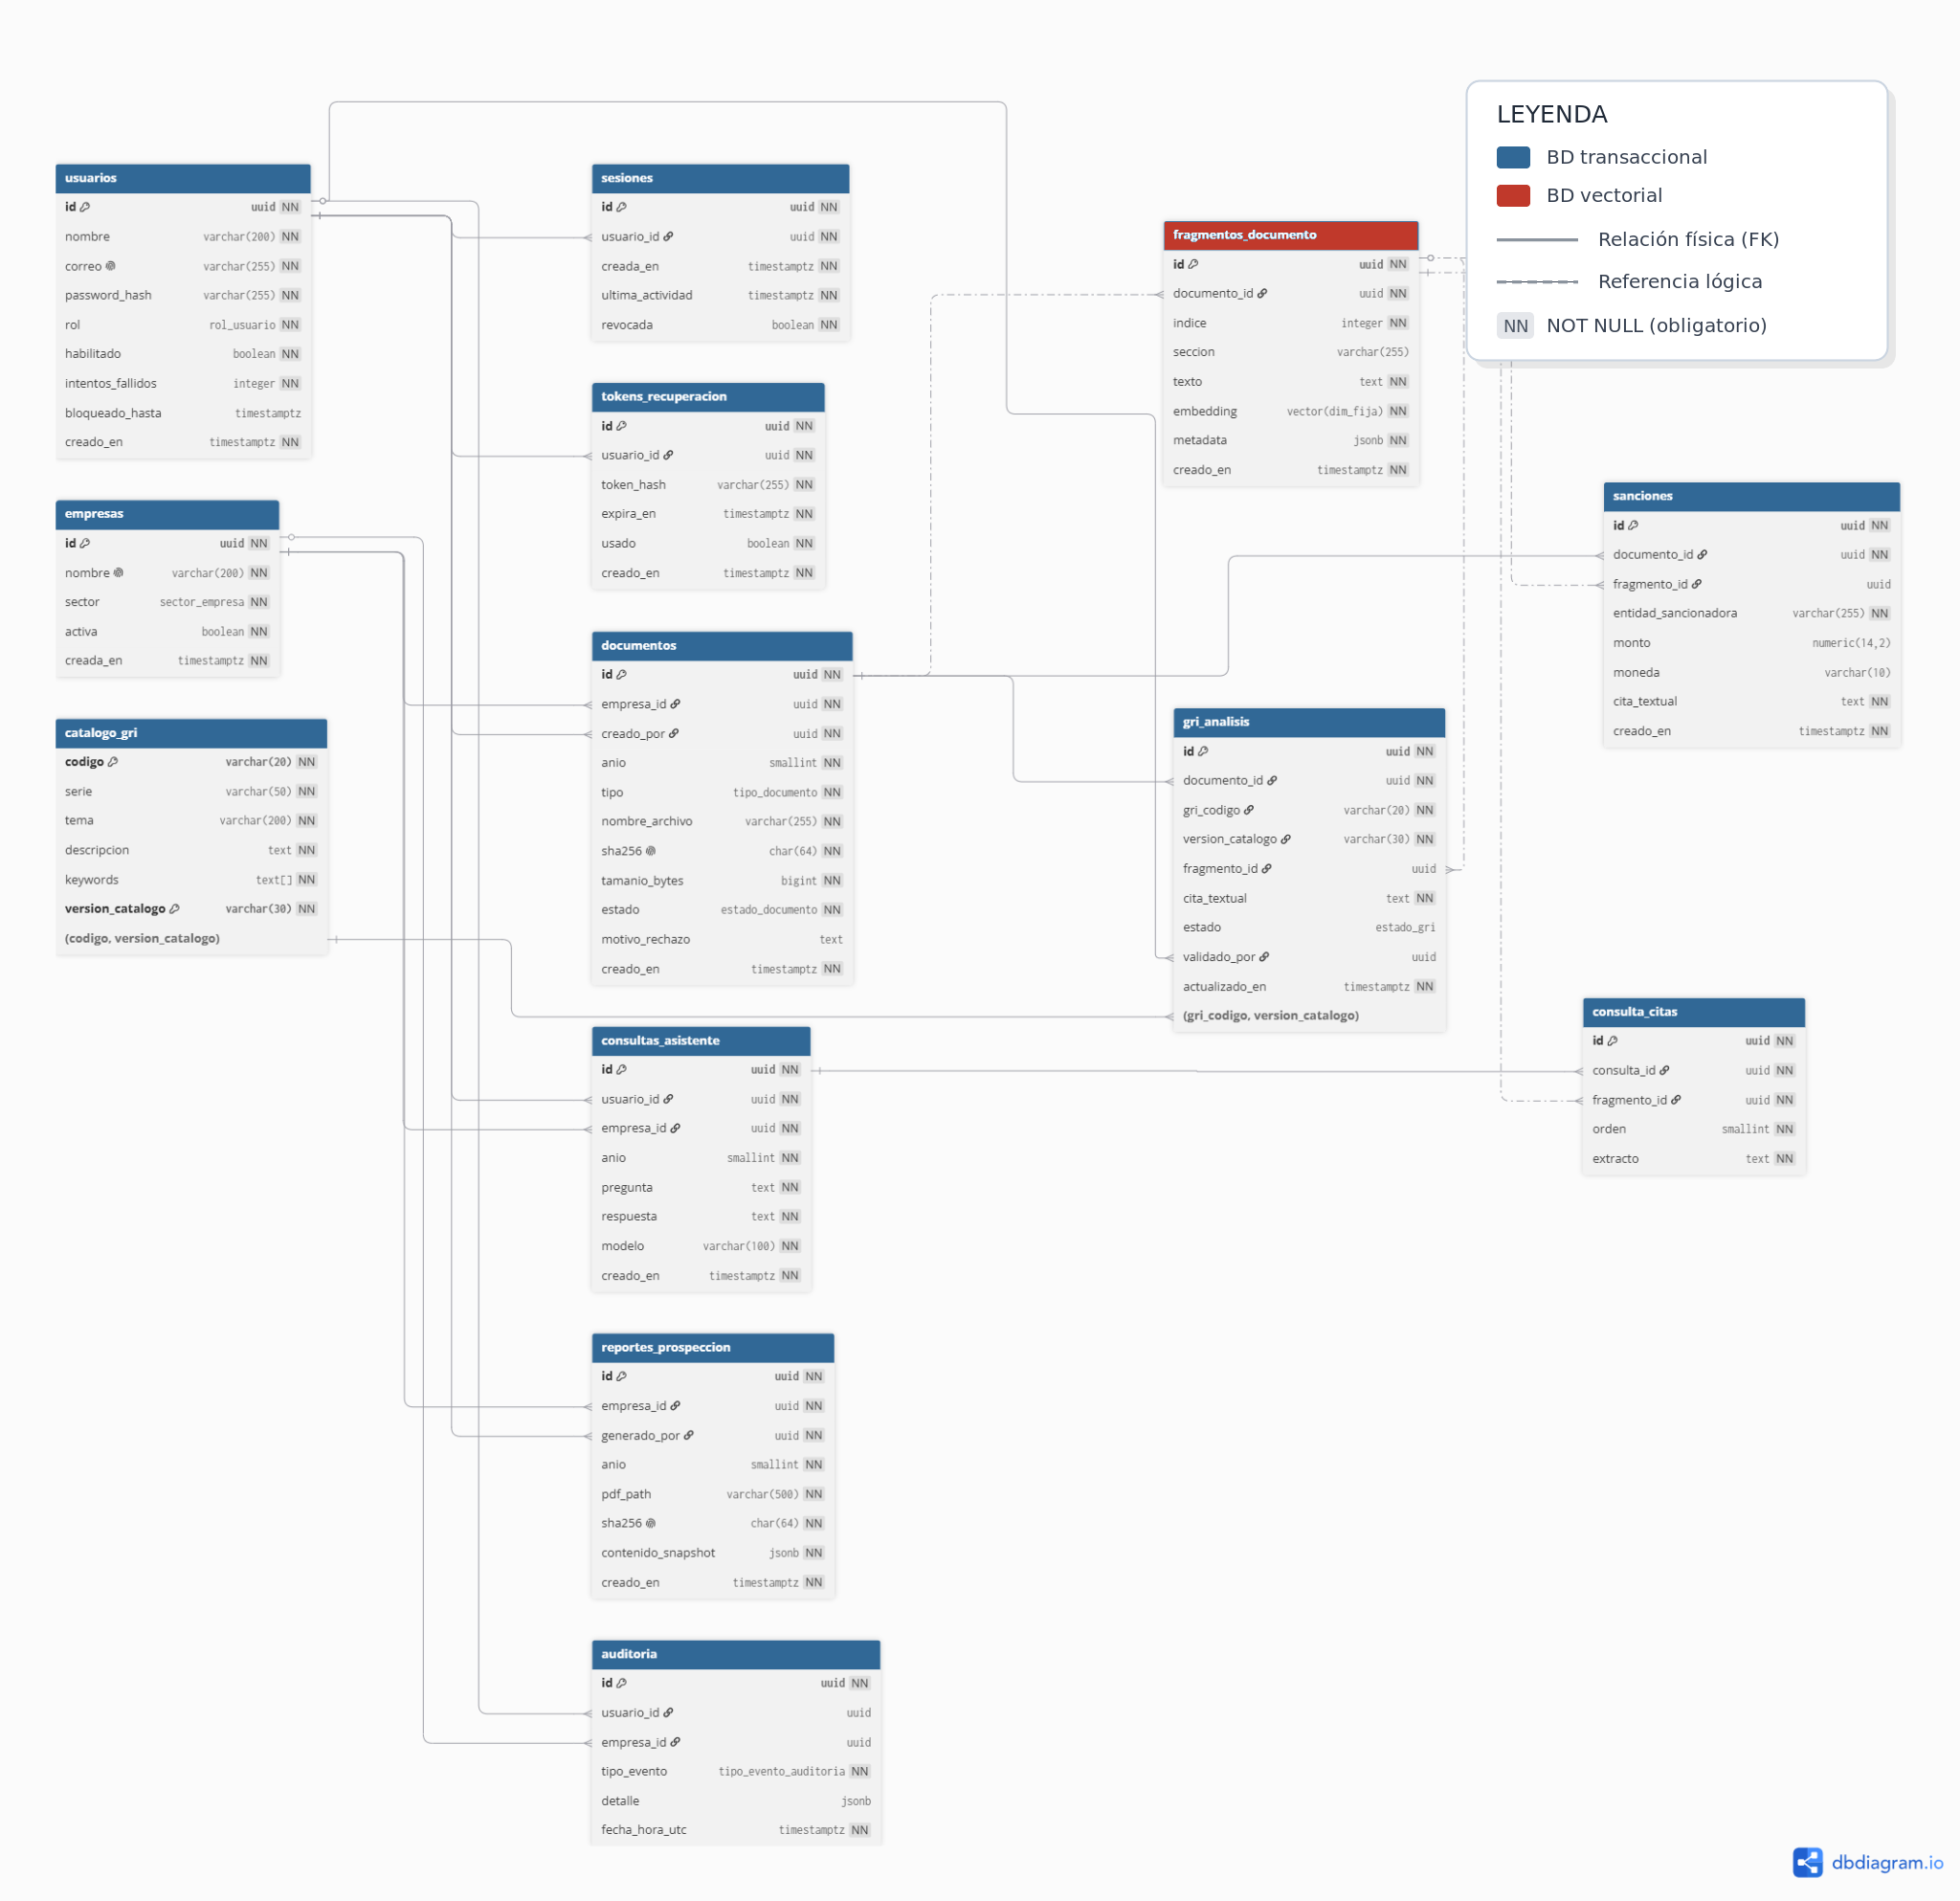
\includegraphics[width=0.95\textwidth]{img/erd-igualab.png}
\end{center}

\subsection{Restricciones clave (UNIQUE y reglas BD)}
\begingroup\small
\begin{longtable}{|L{6.9cm}|L{8.0cm}|}
\hline
\thd{Restricción} & \thd{Descripción} \\
\hline
\endhead
UNIQUE parcial en usuarios.rol (WHERE rol='superadmin') & Un solo Superadmin en toda la tabla --- la transferencia es transacción doble atómica (RS-01). \\
\hline
UNIQUE case-insensitive usuarios.correo (índice lower(correo)) & Correo único de dominio autorizado (RN-007). \\
\hline
UNIQUE documentos.sha256 & El mismo contenido nunca se ingesta dos veces (RNF-011). \\
\hline
UNIQUE parcial (empresa\_id, anio, tipo) WHERE estado='indexado' & Unicidad documental por empresa/año/tipo --- solo para documentos exitosos. \\
\hline
UNIQUE (documento\_id, indice) en fragmentos\_documento & Posición única del fragmento dentro del documento. \\
\hline
UNIQUE parcial (documento\_id, gri\_codigo) en gri\_analisis & Una sola fila de resultados por documento/código. \\
\hline
UNIQUE parcial (empresa\_id, anio) en reportes\_prospeccion & Un solo reporte por empresa/año (RN-041). \\
\hline
CHECK sectores cerrados en empresas.sector & Minería · Petróleo y Gas · Energía (RN-015, en la BD). \\
\hline
CHECK tamano\_bytes $\leq$ 50 MB en documentos & Límite de tamaño (RN-015). \\
\hline
CHECK estados ENUM & estado\_ingesta, estado\_gri, estado\_documental, tipo\_evento\_auditoria. \\
\hline
REVOKE UPDATE, DELETE en auditoria & Append-only garantizado por la BD. \\
\hline
\end{longtable}
\endgroup

\subsection{Tablas retiradas (se quitaron módulos)}
\begin{center}
\begin{tabular}{|L{4.4cm}|L{10.5cm}|}
\hline
\thd{Retirada} & \thd{Justificación} \\
\hline
roles & Catálogo cerrado de 2 filas --- sustituido por ENUM rol\_usuario + UNIQUE parcial en usuarios.rol. \\
\hline
configuracion & La tabla fue retirada; los umbrales operativos se gestionan por variables de entorno (doc Stack §4). \\
\hline
uso\_llm & El consumo diario se deriva de consultas\_asistente (COUNT por día/modelo). \\
\hline
gri\_analisis\_historico & Los cambios sensibles quedan en auditoria (AJUSTE\_BRECHA detalle JSONB). \\
\hline
reporte\_detalle\_snapshot & Sustituida por contenido\_snapshot JSONB + PDF inmutable con hash. \\
\hline
\end{tabular}
\end{center}

\subsection{Decisiones del modelo}
\begin{enumerate}[leftmargin=1.6em,itemsep=2pt,topsep=2pt]
  \item \textbf{8.7.1.} Sectores cerrados: Minería, Petróleo y Gas, Energía (CHECK en la BD).
  \item \textbf{8.7.2.} Estado GRI asignado manualmente por el Administrador: no existe estado\_sugerido.
  \item \textbf{8.7.3.} Sanciones enlazadas al documento; empresa y año se derivan de él (sin duplicar FKs).
  \item \textbf{8.7.4.} Embeddings almacenados en fragmentos\_documento; la dimensión depende del modelo del proveedor (fijar en migración, p. ej. 1024).
  \item \textbf{8.7.5.} Reporte consolidado en JSONB + PDF inmutable (sin tabla normalizada de detalle).
  \item \textbf{8.7.6.} Auditoría unipersonal separada del logging técnico y con modo append-only.
  \item \textbf{8.7.7.} FK de auditoría/consultas visibles en el diagrama (líneas largas omitidas por legibilidad).
\end{enumerate}

% ====================================================================
\section{Diccionario de Datos}

El modelo contiene 12 tablas en la base de datos transaccional y 1 tabla en la base de datos vectorial. Las relaciones entre ambas bases se registran como referencias lógicas (REF), no como claves foráneas físicas.

\newcommand{\dicthead}{\hline \thd{Campo} & \thd{Tamaño} & \thd{Tipo de Dato} & \thd{Descripción} & \thd{NULL} \\ \hline}
\newcommand{\dt}[5]{#1 & #2 & #3 & #4 & #5 \\ \hline}
\newcommand{\tabname}[1]{\par\vspace{10pt}\noindent\textbf{Tabla: #1}\par}

\par\vspace{8pt}\noindent\textbf{Base de datos transaccional:}

\tabname{usuarios}
Descripción: Almacena las cuentas de usuario, sus credenciales, rol y estado de acceso al sistema.
\begingroup\small
\begin{longtable}{|L{2.3cm}|C{1.3cm}|L{2.7cm}|L{6.4cm}|C{1.0cm}|}
\dicthead
\dt{id}{36}{UUID (PK)}{Identificador único del usuario.}{NO}
\dt{nombre}{200}{VARCHAR}{Nombre completo del usuario.}{NO}
\dt{correo}{255}{VARCHAR (UQ)}{Correo electrónico único utilizado para el inicio de sesión.}{NO}
\dt{password\_hash}{255}{VARCHAR}{Hash seguro de la contraseña del usuario.}{NO}
\dt{rol}{-}{rol\_usuario}{Rol asignado al usuario, por ejemplo SUPERADMIN o ADMIN.}{NO}
\dt{habilitado}{-}{BOOLEAN}{Indica si la cuenta está habilitada para acceder al sistema.}{NO}
\dt{intentos\_fallidos}{-}{INTEGER}{Cantidad acumulada de intentos fallidos de autenticación.}{NO}
\dt{bloqueado\_hasta}{-}{TIMESTAMPTZ}{Fecha y hora hasta la que la cuenta permanece bloqueada.}{SÍ}
\dt{creado\_en}{-}{TIMESTAMPTZ}{Fecha y hora de creación de la cuenta.}{NO}
\end{longtable}
\endgroup

\tabname{sesiones}
Descripción: Registra las sesiones iniciadas por los usuarios y permite controlar su actividad y revocación.
\begingroup\small
\begin{longtable}{|L{2.3cm}|C{1.3cm}|L{2.7cm}|L{6.4cm}|C{1.0cm}|}
\dicthead
\dt{id}{36}{UUID (PK)}{Identificador único de la sesión.}{NO}
\dt{usuario\_id}{36}{UUID (FK)}{Usuario propietario de la sesión. Referencia a usuarios.id.}{NO}
\dt{creada\_en}{-}{TIMESTAMPTZ}{Fecha y hora en que se creó la sesión.}{NO}
\dt{ultima\_actividad}{-}{TIMESTAMPTZ}{Fecha y hora de la actividad más reciente de la sesión.}{NO}
\dt{revocada}{-}{BOOLEAN}{Indica si la sesión fue invalidada antes de su expiración.}{NO}
\end{longtable}
\endgroup

\tabname{tokens\_recuperacion}
Descripción: Almacena los tokens de recuperación de contraseña y controla su vigencia y utilización.
\begingroup\small
\begin{longtable}{|L{2.3cm}|C{1.3cm}|L{2.7cm}|L{6.4cm}|C{1.0cm}|}
\dicthead
\dt{id}{36}{UUID (PK)}{Identificador único del token de recuperación.}{NO}
\dt{usuario\_id}{36}{UUID (FK)}{Usuario que solicitó la recuperación. Referencia a usuarios.id.}{NO}
\dt{token\_hash}{255}{VARCHAR (IDX)}{Hash del token enviado al usuario; se indexa para facilitar su búsqueda.}{NO}
\dt{expira\_en}{-}{TIMESTAMPTZ}{Fecha y hora de vencimiento del token.}{NO}
\dt{usado}{-}{BOOLEAN}{Indica si el token ya fue utilizado.}{NO}
\dt{creado\_en}{-}{TIMESTAMPTZ}{Fecha y hora de creación del token.}{NO}
\end{longtable}
\endgroup
Reglas semánticas: expirado o ya usado deriva a inválido. La contraseña nueva revoca todas las sesiones del usuario.

\tabname{empresas}
Descripción: Contiene las empresas evaluadas por la plataforma y la información básica de su clasificación.
\begingroup\small
\begin{longtable}{|L{2.3cm}|C{1.3cm}|L{2.7cm}|L{6.4cm}|C{1.0cm}|}
\dicthead
\dt{id}{36}{UUID (PK)}{Identificador único de la empresa.}{NO}
\dt{nombre}{200}{VARCHAR (UQ)}{Nombre único de la empresa.}{NO}
\dt{sector}{-}{sector\_empresa}{Sector económico al que pertenece la empresa.}{NO}
\dt{activa}{-}{BOOLEAN}{Indica si la empresa se encuentra activa en el sistema.}{NO}
\dt{creada\_en}{-}{TIMESTAMPTZ}{Fecha y hora de registro de la empresa.}{NO}
\end{longtable}
\endgroup

\tabname{documentos}
Descripción: Registra los documentos cargados para una empresa y controla su identificación, integridad y estado de procesamiento.
\begingroup\small
\begin{longtable}{|L{2.3cm}|C{1.3cm}|L{2.7cm}|L{6.4cm}|C{1.0cm}|}
\dicthead
\dt{id}{36}{UUID (PK)}{Identificador único del documento.}{NO}
\dt{empresa\_id}{36}{UUID (FK)}{Empresa a la que pertenece el documento. Referencia a empresas.id.}{NO}
\dt{creado\_por}{36}{UUID (FK)}{Usuario que registró el documento. Referencia a usuarios.id.}{NO}
\dt{anio}{-}{SMALLINT}{Año al que corresponde el documento.}{NO}
\dt{tipo}{-}{tipo\_documento}{Tipo de documento cargado.}{NO}
\dt{nombre\_archivo}{255}{VARCHAR}{Nombre original del archivo cargado.}{NO}
\dt{sha256}{64}{CHAR (UQ)}{Huella SHA-256 única utilizada para validar integridad y evitar duplicados.}{NO}
\dt{tamanio\_bytes}{-}{BIGINT}{Tamaño del archivo expresado en bytes.}{NO}
\dt{estado}{-}{estado\_documento}{Estado del documento dentro del flujo de ingesta y análisis.}{NO}
\dt{motivo\_rechazo}{-}{TEXT}{Motivo del rechazo cuando el documento no puede ser procesado.}{SÍ}
\dt{creado\_en}{-}{TIMESTAMPTZ}{Fecha y hora de registro del documento.}{NO}
\end{longtable}
\endgroup

\tabname{catalogo\_gri}
Descripción: Mantiene el catálogo versionado de estándares e indicadores GRI utilizados en el análisis documental.
\begingroup\small
\begin{longtable}{|L{2.3cm}|C{1.3cm}|L{2.7cm}|L{6.4cm}|C{1.0cm}|}
\dicthead
\dt{codigo}{20}{VARCHAR (PK*)}{Código del estándar GRI. Forma la clave primaria compuesta con version\_catalogo.}{NO}
\dt{serie}{50}{VARCHAR}{Serie a la que pertenece el estándar GRI.}{NO}
\dt{tema}{200}{VARCHAR}{Tema o denominación del estándar GRI.}{NO}
\dt{descripcion}{-}{TEXT}{Descripción funcional del estándar o indicador.}{NO}
\dt{keywords}{-}{TEXT ARRAY}{Palabras clave utilizadas para apoyar la identificación del estándar.}{NO}
\dt{version\_catalogo}{30}{VARCHAR (PK*)}{Versión del catálogo. Forma la clave primaria compuesta con codigo.}{NO}
\end{longtable}
\endgroup

\tabname{gri\_analisis}
Descripción: Almacena los resultados del análisis GRI identificados en cada documento y su eventual validación.
\begingroup\small
\begin{longtable}{|L{2.3cm}|C{1.3cm}|L{2.7cm}|L{6.4cm}|C{1.0cm}|}
\dicthead
\dt{id}{36}{UUID (PK)}{Identificador único del resultado de análisis GRI.}{NO}
\dt{documento\_id}{36}{UUID (FK)}{Documento analizado. Referencia a documentos.id.}{NO}
\dt{gri\_codigo}{20}{VARCHAR (FK*)}{Código GRI; integra la clave foránea compuesta hacia catalogo\_gri.}{NO}
\dt{version\_catalogo}{30}{VARCHAR (FK*)}{Versión del catálogo; integra la clave foránea compuesta hacia catalogo\_gri.}{NO}
\dt{fragmento\_id}{36}{UUID (REF)}{Referencia lógica al fragmento que sustenta el hallazgo en fragmentos\_documento.id.}{SÍ}
\dt{cita\_textual}{-}{TEXT}{Texto del documento utilizado como evidencia del hallazgo.}{NO}
\dt{estado}{-}{estado\_gri}{Estado de revisión o validación del resultado GRI.}{SÍ}
\dt{validado\_por}{36}{UUID (FK)}{Usuario que validó el resultado. Referencia a usuarios.id.}{SÍ}
\dt{actualizado\_en}{-}{TIMESTAMPTZ}{Fecha y hora de la última actualización del resultado.}{NO}
\end{longtable}
\endgroup

\tabname{sanciones}
Descripción: Registra las sanciones detectadas en los documentos y conserva la evidencia textual asociada.
\begingroup\small
\begin{longtable}{|L{2.4cm}|C{1.2cm}|L{2.6cm}|L{6.5cm}|C{1.0cm}|}
\dicthead
\dt{id}{36}{UUID (PK)}{Identificador único de la sanción.}{NO}
\dt{documento\_id}{36}{UUID (FK)}{Documento donde se identificó la sanción. Referencia a documentos.id.}{NO}
\dt{fragmento\_id}{36}{UUID (REF)}{Referencia lógica al fragmento de evidencia en fragmentos\_documento.id.}{SÍ}
\dt{entidad\_sancionadora}{255}{VARCHAR}{Nombre de la entidad que impuso la sanción.}{NO}
\dt{monto}{14,2}{NUMERIC}{Importe monetario asociado a la sanción.}{SÍ}
\dt{moneda}{10}{VARCHAR}{Código o denominación de la moneda del monto registrado.}{SÍ}
\dt{cita\_textual}{-}{TEXT}{Texto del documento que sustenta la sanción identificada.}{NO}
\dt{creado\_en}{-}{TIMESTAMPTZ}{Fecha y hora de registro de la sanción.}{NO}
\end{longtable}
\endgroup

\tabname{consultas\_asistente}
Descripción: Registra las preguntas realizadas al asistente RAG, sus respuestas y el contexto de consulta.
\begingroup\small
\begin{longtable}{|L{2.3cm}|C{1.3cm}|L{2.7cm}|L{6.4cm}|C{1.0cm}|}
\dicthead
\dt{id}{36}{UUID (PK)}{Identificador único de la consulta.}{NO}
\dt{usuario\_id}{36}{UUID (FK)}{Usuario que realizó la consulta. Referencia a usuarios.id.}{NO}
\dt{empresa\_id}{36}{UUID (FK)}{Empresa utilizada como contexto. Referencia a empresas.id.}{NO}
\dt{anio}{-}{SMALLINT}{Año utilizado como filtro de la consulta.}{NO}
\dt{pregunta}{-}{TEXT}{Pregunta formulada por el usuario.}{NO}
\dt{respuesta}{-}{TEXT}{Respuesta generada por el asistente.}{NO}
\dt{modelo}{100}{VARCHAR}{Modelo de inteligencia artificial utilizado para generar la respuesta.}{NO}
\dt{creado\_en}{-}{TIMESTAMPTZ}{Fecha y hora de ejecución de la consulta.}{NO}
\end{longtable}
\endgroup

\tabname{consulta\_citas}
Descripción: Relaciona cada respuesta del asistente con los fragmentos documentales utilizados como citas o evidencia.
\begingroup\small
\begin{longtable}{|L{2.3cm}|C{1.3cm}|L{2.7cm}|L{6.4cm}|C{1.0cm}|}
\dicthead
\dt{id}{36}{UUID (PK)}{Identificador único de la cita.}{NO}
\dt{consulta\_id}{36}{UUID (FK)}{Consulta a la que pertenece la cita. Referencia a consultas\_asistente.id.}{NO}
\dt{fragmento\_id}{36}{UUID (REF)}{Referencia lógica al fragmento citado en fragmentos\_documento.id.}{NO}
\dt{orden}{-}{SMALLINT}{Posición de la cita dentro de la respuesta.}{NO}
\dt{extracto}{-}{TEXT}{Extracto presentado como evidencia en la respuesta.}{NO}
\end{longtable}
\endgroup

\tabname{reportes\_prospeccion}
Descripción: Almacena los reportes de prospección generados para cada empresa y año, junto con su contenido consolidado.
\begingroup\small
\begin{longtable}{|L{2.3cm}|C{1.3cm}|L{2.7cm}|L{6.4cm}|C{1.0cm}|}
\dicthead
\dt{id}{36}{UUID (PK)}{Identificador único del reporte de prospección.}{NO}
\dt{empresa\_id}{36}{UUID (FK/UQ*)}{Empresa del reporte. Forma una restricción única compuesta con anio.}{NO}
\dt{generado\_por}{36}{UUID (FK)}{Usuario que generó el reporte. Referencia a usuarios.id.}{NO}
\dt{anio}{-}{SMALLINT (UQ*)}{Año del reporte. Forma una restricción única compuesta con empresa\_id.}{NO}
\dt{pdf\_path}{500}{VARCHAR}{Ruta de almacenamiento del archivo PDF generado.}{NO}
\dt{sha256}{64}{CHAR (UQ)}{Huella SHA-256 única del reporte para verificar su integridad.}{NO}
\dt{contenido\_snapshot}{-}{JSONB}{Instantánea de los datos utilizados para generar el reporte.}{NO}
\dt{creado\_en}{-}{TIMESTAMPTZ}{Fecha y hora de generación del reporte.}{NO}
\end{longtable}
\endgroup

\tabname{auditoria}
Descripción: Registra eventos relevantes del sistema para fines de trazabilidad, control y revisión.
\begingroup\small
\begin{longtable}{|L{2.3cm}|C{1.3cm}|L{2.7cm}|L{6.4cm}|C{1.0cm}|}
\dicthead
\dt{id}{36}{UUID (PK)}{Identificador único del evento de auditoría.}{NO}
\dt{usuario\_id}{36}{UUID (FK)}{Usuario relacionado con el evento. Referencia a usuarios.id.}{SÍ}
\dt{empresa\_id}{36}{UUID (FK)}{Empresa relacionada con el evento. Referencia a empresas.id.}{SÍ}
\dt{tipo\_evento}{-}{tipo\_evento\_auditoria}{Clasificación del evento registrado.}{NO}
\dt{detalle}{-}{JSONB}{Información adicional y estructurada del evento.}{SÍ}
\dt{fecha\_hora\_utc}{-}{TIMESTAMPTZ}{Fecha y hora UTC en que ocurrió el evento.}{NO}
\end{longtable}
\endgroup

\par\vspace{8pt}\noindent\textbf{Base de datos vectorial:}

\tabname{fragmentos\_documento}
Descripción: Almacena los fragmentos extraídos de los documentos, sus embeddings y metadatos para la recuperación semántica.
\begingroup\small
\begin{longtable}{|L{2.3cm}|C{1.3cm}|L{2.7cm}|L{6.4cm}|C{1.0cm}|}
\dicthead
\dt{id}{36}{UUID (PK)}{Identificador único del fragmento vectorial.}{NO}
\dt{documento\_id}{36}{UUID (REF)}{Referencia lógica al documento de origen en documentos.id, ubicado en la base transaccional.}{NO}
\dt{indice}{-}{INTEGER (UQ*)}{Posición del fragmento dentro del documento; es única en combinación con documento\_id.}{NO}
\dt{seccion}{255}{VARCHAR}{Sección o encabezado del documento al que pertenece el fragmento.}{SÍ}
\dt{texto}{-}{TEXT}{Contenido textual completo del fragmento.}{NO}
\dt{embedding}{dim\_fija}{VECTOR}{Representación vectorial del texto generada por el proveedor de embeddings.}{NO}
\dt{metadata}{-}{JSONB}{Metadatos estructurados asociados al fragmento.}{NO}
\dt{creado\_en}{-}{TIMESTAMPTZ}{Fecha y hora de creación del fragmento.}{NO}
\end{longtable}
\endgroup

% ====================================================================
\section{Volumen Estimado}
La siguiente tabla presenta una estimación del volumen mensual de datos generado por cada módulo del sistema. Los valores son referenciales y permiten identificar los módulos con mayor demanda de almacenamiento y procesamiento.

\begin{center}
\begin{tabular}{|L{4.6cm}|C{3.0cm}|C{1.5cm}|L{5.6cm}|}
\hline
\thd{Módulo} & \thd{Volumen estimado} & \thd{Nivel} & \thd{Justificación} \\
\hline
Autenticación y Gestión de Sesión & 170 registros & Medio & Considera aproximadamente 168 sesiones y 2 solicitudes de recuperación de contraseña al mes. \\
\hline
Gestión de Usuarios & 4 a 6 cuentas activas & Bajo & Referencia lógica al documento de origen en documentos.id, ubicado en la base transaccional. \\
\hline
Catálogo de Empresas & 8 a 10 empresas & Bajo & Corresponde al registro progresivo de empresas habilitadas para el análisis. \\
\hline
Ingesta de Documentos & 42 documentos y 4,200 fragmentos & Alto & Cada documento se divide en aproximadamente 100 fragmentos con embeddings para su almacenamiento en la base vectorial. \\
\hline
Análisis y Validación de Brechas GRI & 425 registros & Medio & Considera aproximadamente 417 resultados de análisis y 8 sanciones identificadas. El catálogo de 40 códigos GRI permanece como información base. \\
\hline
Asistente de Inteligencia Artificial (RAG) & 1,670 registros & Alto & Considera aproximadamente 420 consultas y 1,250 citas, con un promedio de tres citas por respuesta. \\
\hline
Generación de Reportes de Prospección & 8 a 10 reportes & Bajo & Los reportes se generan únicamente para empresas con información analizada y validada. \\
\hline
Auditoría Funcional & 420 eventos & Medio & Registra accesos, cambios de usuarios, ingestas, rechazos de documentos y generación de reportes. \\
\hline
\end{tabular}
\end{center}

% ====================================================================
\section{Diseño Arquitectónico}
La solución se estructura como una arquitectura de solución por capas, con dependencias unidireccionales de arriba hacia abajo (cada capa invoca únicamente a la inmediata inferior). Las siete capas son: actores y roles; aplicación web (SPA React 18 + Vite); API REST (FastAPI); servicios y lógica de negocio (Python 3.11, monolito modular); procesamiento y reglas por módulo; persistencia (SQLAlchemy Async); y base de datos PostgreSQL 16 con la extensión pgvector. La separación por capas y la modularidad interna (principios SOLID, con un único servicio por módulo) se detallan en la sección 4. La figura siguiente presenta el diagrama de arquitectura de solución por capas.

\begin{center}
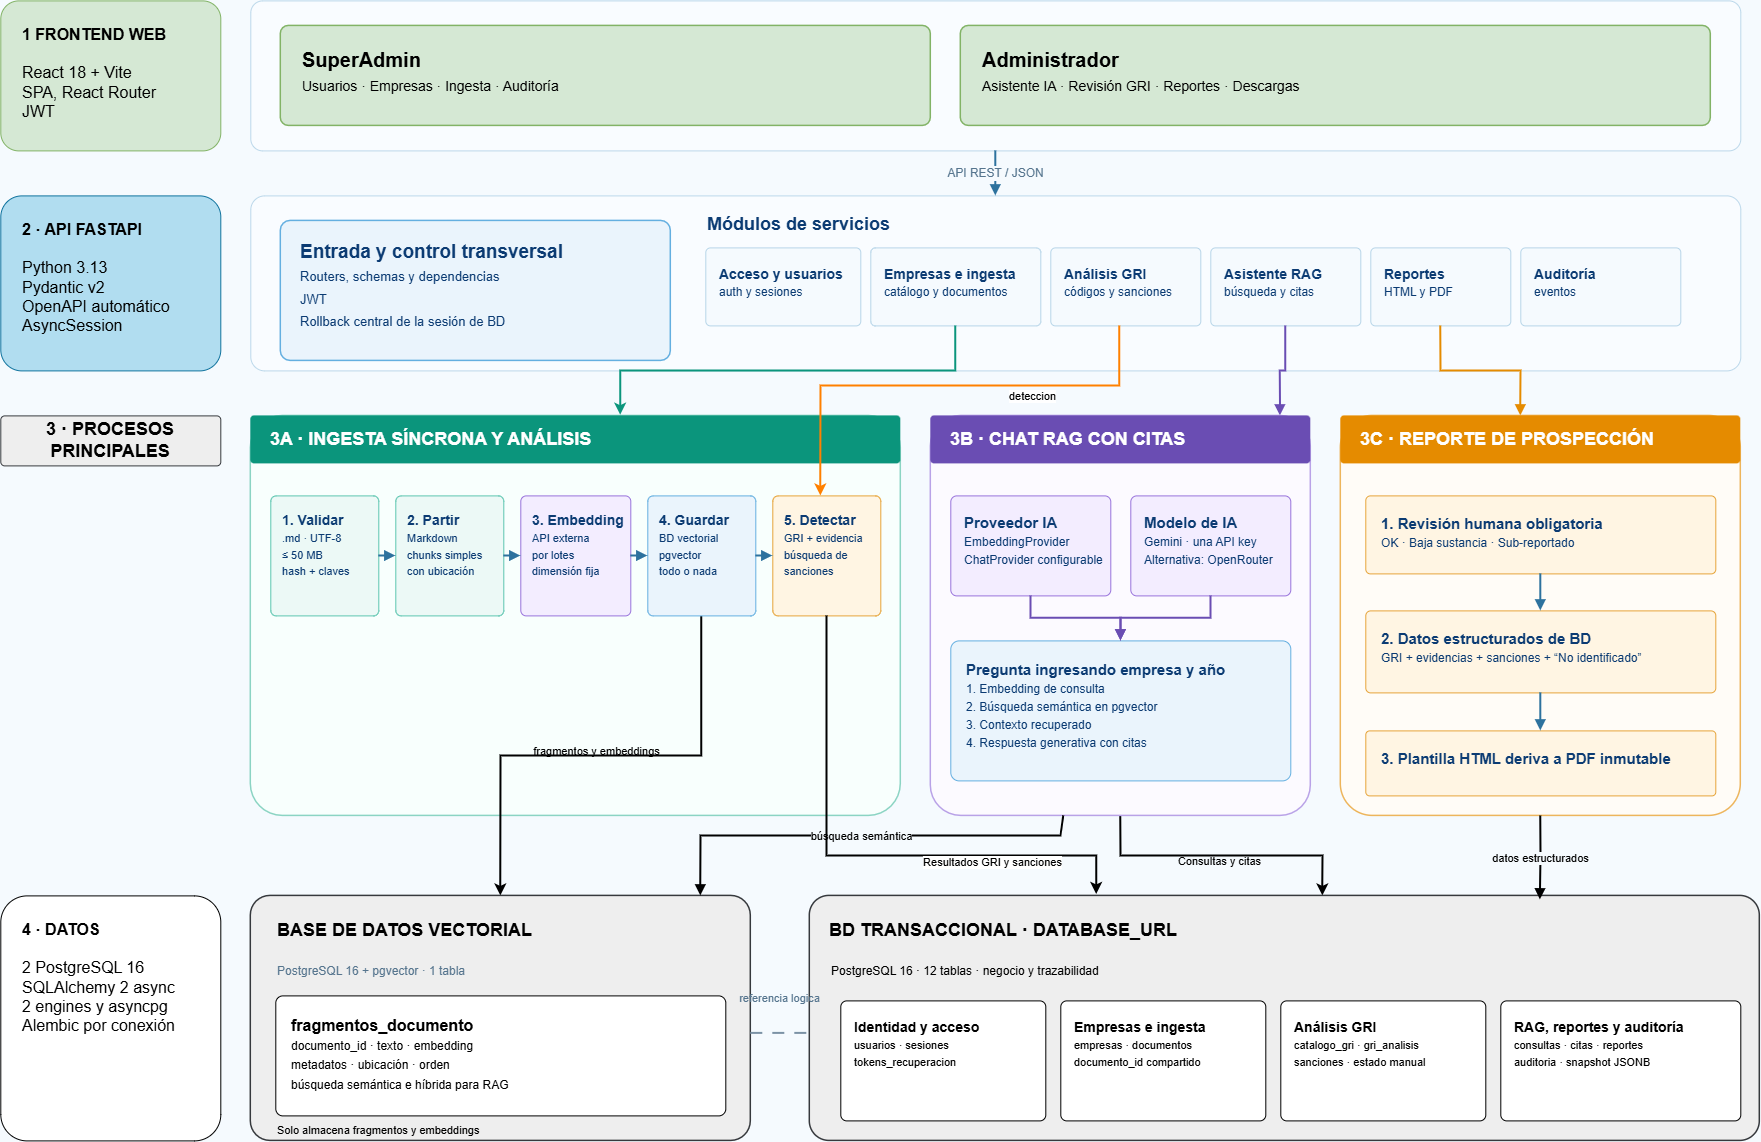
\includegraphics[width=0.98\textwidth]{img/arquitectura-igualab.png}
\end{center}

\section{Prototipo}
El prototipo navegable de la FASE 1 está disponible e implementa las pantallas de los módulos descritos en este documento (autenticación, gestión de usuarios, catálogo de empresas e ingesta, asistente de IA, reportes de prospección y auditoría), organizadas por rol: el SuperAdmin accede a la gestión de usuarios, la ingesta y la auditoría; el Administrador, al asistente de IA, los reportes y las descargas.

\section{Anexo}
\subsection{Problemas identificados del proceso actual (AS-IS)}
A partir del análisis del proceso actual (AS-IS) se identifican los siguientes problemas. El analista de Igualab debe buscar y descargar manualmente cada informe (memoria anual y/o reporte de sostenibilidad) de fuentes dispersas, lo que incrementa el riesgo de omitir documentos relevantes o descargar versiones desactualizadas. La revisión íntegra de documentos que suelen exceder las 100 páginas depende enteramente de su criterio individual, lo que genera variabilidad en la cobertura y profundidad del análisis entre distintas revisiones. No existe un catálogo estandarizado de indicadores GRI evaluables ni una metodología uniforme para asignar estados de cumplimiento, por lo que los criterios pueden variar de una empresa a otra. Una vez identificadas brechas, sanciones o hallazgos, el analista no registra la información en un sistema estructurado ni base de datos, ni hoja de cálculo, ni herramienta similar, por lo que los resultados quedan en su conocimiento implícito, sin posibilidad de consulta histórica, comparación entre empresas o trazabilidad. Tampoco se registra qué empresa revisó, en qué fecha ni con qué criterios, lo que impide validar la calidad del análisis o demostrar diligencia ante el cliente. La elaboración del documento de prospección se realiza en texto libre sin plantilla estandarizada, lo que genera formatos inconsistentes y omisión de información relevante. En conjunto, cada análisis parte de cero y no permite reutilizar resultados previos, comparar evolución año a año ni escalar el proceso a más empresas sin incrementar linealmente la carga de trabajo.

\subsection{Matriz de trazabilidad (módulo · CU · RF · RN · RNF)}
La matriz siguiente consolida la cobertura de cada módulo funcional: su caso de uso, los requerimientos funcionales que implementa y su respaldo en reglas de negocio y requerimientos no funcionales.

\begin{center}
\begingroup\small
\begin{longtable}{|C{0.7cm}|L{3.8cm}|C{1.3cm}|L{4.6cm}|L{4.3cm}|}
\hline
\thd{\#} & \thd{Módulo} & \thd{CU} & \thd{Requerimientos Funcionales (RF)} & \thd{Respaldo (RN · RNF)} \\
\hline
\endhead
1 & Autenticación y Gestión de Sesión & CU001 & RF-001…RF-005 & RN-004…RN-013 · RNF-001…RNF-009 \\
\hline
2 & Gestión de Usuarios & CU002 & RF-006…RF-009 & RN-001…RN-009 · RNF-012, RNF-013 \\
\hline
3 & Catálogo de Empresas & CU003 & RF-010, RF-011 & RN-014…RN-017 \\
\hline
4 & Ingesta de Documentos & CU003 & RF-012…RF-017 & RN-018…RN-026 · RNF-007, RNF-011, RNF-015, RNF-016, RNF-020, RNF-025, RNF-029 \\
\hline
5 & Análisis y Validación de Brechas GRI & CU005 & RF-018…RF-022, RF-028 & RN-027…RN-032 · RNF-014, RNF-026, RNF-027 \\
\hline
6 & Asistente de IA (RAG) & CU004 & RF-023, RF-024 & RN-033…RN-037 · RNF-010, RNF-017, RNF-018, RNF-019 \\
\hline
7 & Generación de Reportes de Prospección & CU006 & RF-025…RF-027 & RN-038…RN-041 \\
\hline
8 & Auditoría Funcional & CU007 & RF-029, RF-030 & RN-042…RN-045 · RNF-022, RNF-023, RNF-024 \\
\hline
\end{longtable}
\endgroup
\end{center}
